\documentclass[11pt]{article}
\usepackage{array, xcolor}
\usepackage[margin=1.5cm]{geometry}
\usepackage{hyperref}

\usepackage{graphicx,mwe}
\usepackage{array}
\usepackage{graphicx}
\usepackage{wrapfig}

\usepackage{enumitem}

\usepackage{fontspec}
\defaultfontfeatures{Scale=MatchLowercase,Mapping=tex-text}
\setmainfont[Ligatures=TeX]{DejaVu Serif}
\setsansfont[Ligatures=TeX]{DejaVu Sans}
\setmonofont{DejaVu Sans Mono}
 
 \usepackage[none]{hyphenat}
  
\title{\bfseries\Huge Oleg Shpynov}
\author{oleg.shpynov@gmail.com}
\date{}
 
\definecolor{lightgray}{gray}{0.8}
\newcolumntype{L}{>{\raggedleft}p{0.14\textwidth}}
\newcolumntype{R}{p{0.8\textwidth}}
\newcommand\VRule{\color{lightgray}\vrule width 0.5pt}
 
%%% Begin Document
\begin{document}
\begin{wrapfigure}{r}{0.3\textwidth}
    \vspace*{-4cm} % moving actual picture up
	\hfill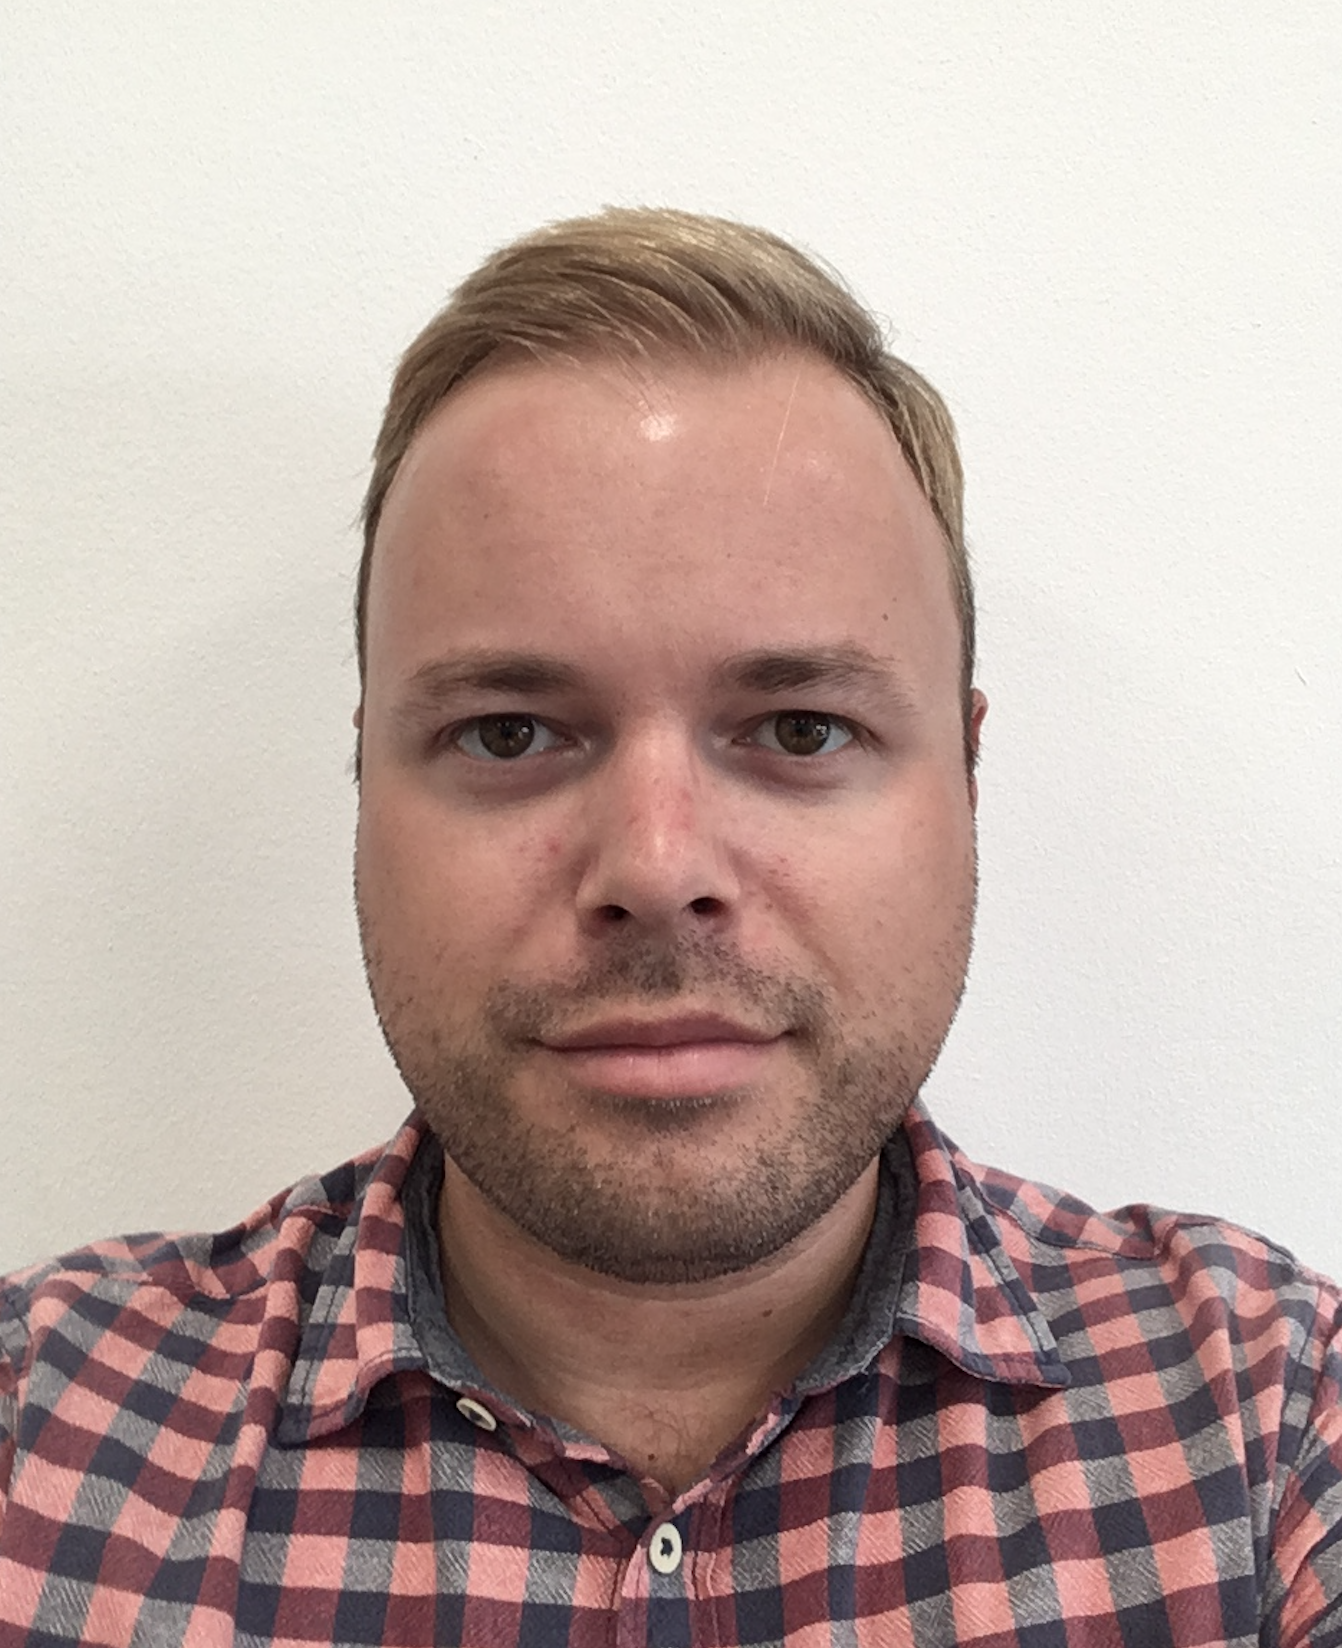
\includegraphics[width=0.20\textwidth]{me2020.png}
    \vspace*{-4cm} % avoid real text wrapping
\end{wrapfigure}

\maketitle 

%%% Personal details
\begin{minipage}[ht]{0.4\textwidth}
Shuvalovsky pr. 84 135\\
Saint-Petersburg\\
Russia\\
197345
\end{minipage}
\begin{minipage}[ht]{0.3\textwidth}
April 7th, 1986\\
+7 904 331 35 04
\end{minipage}
\vspace{10pt}

%%% About me short
\section*{Summary}
Seasoned research engineering leader with strong math background, good communication and teamwork skills.\\
I am leading a group that develops machine learning algorithms and scalable computational  bioinformatics pipelines for biological data analysis. Previously I was focused on Integrated Development Environment development from lexical analysis to advanced type systems development and semantic verifications.

%%% Professional experience
\section*{Experience}
\begin{tabular}{L!{\VRule}R}
2013 -- today & \textbf{Research and Development Team Lead}\\
& \textit{JetBrains Research, Saint-Petersburg, Russia}\\[5pt]
& Head of research and development bioinformatics group. Group is developing novel algorithms and methods for experimental data analysis, building scalable computational pipelines and tools, and working in collaboration with biologists on various ageing studies.\\
& \setlist{nolistsep}

\begin{itemize}[noitemsep]
	\item Built a team of software developers with expertise in machine learning and bioinformatics
	\item Lead development of two bioinformatics products: \href{https://research.jetbrains.org/groups/biolabs/tools/jbr-genome-browser}{JBR Genome Browser} and \href{https://research.jetbrains.org/groups/biolabs/tools/span-peak-analyzer}{SPAN Semi-supervised Peak Analyzer}
	\item Developed various open source libraries including Viktor (fast f64 computations for Kotlin), Bioinf-commons (Bioinformatics library in Koltin), big (BigBed/Wig files format support for JVM), npy (Numpy arrays support for JVM)
	\item Onboarding and mentoring software developers of all levels
	\item Coordinated research and development activities in collaborations with biologists
	\item Developed scientific papers search and analyze service \href{https://research.jetbrains.org/groups/biolabs/projects?project_id=56}{PubTrends}
\end{itemize}\\
& Applied technologies: Unix, Java, Kotlin, Swing, Python, Jupyter, Pandas, Matplotlib, Docker, Docker Compose, PostgreSQL, Neo4j, Flask, Celery, Nltk, Pytorch, HTML, CSS, Javascript, React, Bootstrap, Git, GitHub, AWS, Continuous Integration TeamCity\\
\\
& Group website: \href{https://research.jetbrains.org/groups/biolabs}{https://research.jetbrains.org/groups/biolabs}\\
& GitHub account: \href{https://github.com/olegs}{https://github.com/olegs}\\
\\
\end{tabular}

\begin{tabular}{L!{\VRule}R}

2014 -- today  & \textbf{Students mentor}\\
& \textit{Computer Science Center, Saint-Petersburg, Russia}\\
& \textit{Higher School of Economics, Saint-Petersburg, Russia}\\
& \textit{Bioinformatics Institute, Saint-Petersburg, Russia}\\
& Mentored various student project in software development and machine learning including two successful Masters dissertations\\
\\

2017 -- 2018 & \textbf{Visiting Research Scientist}\\
& \textit{Department of Pathology and Immunology, Washington University School of Medicine,} \\
& \textit{St. Louis, MO, USA}\\[5pt]
& Computational lead in a joint project of Maxim Artyomov Lab at Washington University in St.Louis . Worked on applied machine learning approaches and methods for epigenetic data analysis.\\
& \setlist{nolistsep}
\begin{itemize}[noitemsep]
	\item Built scalable high-performance computational pipelines targeting Portable Batch System
	\item Analyzed data for various biological experimental
	\item Created web resource portals for experimental data
\end{itemize}\\

& Applied technologies: Unix, QSUB, Bash, Snakemake, Java, Kotlin, Python, Jupyter, Pandas, Matplotlib, Pytest, Git, Docker, Continuous Integration TeamCity, HTML, CSS, Javascript, Bootstrap, Word, Excel, Adobe Illustrator\\
\\
& Project website: \href{https://artyomovlab.wustl.edu/aging}{https://artyomovlab.wustl.edu/aging}\\
\\

2006 -- 2013 & \textbf{Senior software developer}\\
& \textit{JetBrains, Saint-Petersburg, Russia}\\[5pt]
& Main focus was on the analysis of source code in programming languages, starting from lexical analysis to advanced type system development and source code semantic verifications.\\

& \setlist{nolistsep}
\begin{itemize}[noitemsep]
	\item Developed JetBrains products: flagship tool \href{https://jetbrains.com/idea}{IntellIJ IDEA}, \href{https://jetbrains.com/pycharm}{PyCharm}
	\item Created \href{http://jetbrains.com/ruby}{RubyMine} Integrated Development Environment for Ruby programming language	
	\item Maintained and developed \href{https://plugins.jetbrains.com/plugin/164?pr=idea}{IdeaVIM} plugin (vim emulation plugin, 7+mln downloads)
	\item Took part in various IntelliJ IDEA plugins development: GitHub integration support, web-markup languages editing capabilities like YAML, SCSS, LESS, etc.
	\item Participated in a number of conferences on Ruby on Rails as a company representative and a speaker
	\item Author of various \href{https://blog.jetbrains.com/ruby/author/oleg_s/}{blog} posts on Rubymine, IntelliJ IDEA, etc.
\end{itemize}\\
& Applied technologies: Ruby, Rails, Unix, Java, Concurrency, IDE, Swing, Git, GitHub, Continuous Integration TeamCity\\
\\
& Website: \href{https://www.jetbrains.com}{https://www.jetbrains.com/}\\
\\

\end{tabular}


%%% Education
\section*{Education}
\begin{tabular}{L!{\VRule}R}
2019 & Deep learning nanodegree at Udacity, certificate number: 9GSNRHUA  \\
& Machine learning, deep learning, models deployment \\ 
& \\
2016 & Systems Biology Workshop by Bioinformatics Institute, University ITMO and Artyomov Lab of Washington University in St.Louis, Saint-Petersburg, Russia \\
& System level data ranging from gene expression, RNA-, ChIP-, and exome-sequencing up to high-throughput metabolomics and network-based data integration.  \\ 
& \\
2015 & Microsoft Machine Learning and Intelligence School, Microsoft, Russia \\
& Machine learning, artificial intelligence, statistics. \\ 
& \\
2011 -- 2012 & Saint-Petersburg Academic University — Nanotechnology Research and Education Centre of the Russian Academy of Sciences, Russia\\
& Classes of bioinformatics, molecular biology, statistics. \\
& \\
2008 -- 2010 & Post graduate student (PhD) in Computer Science, Faculty of Mathematics and Mechanics, Saint-Petersburg State University, Russia \\
& \\
2003 -- 2008 & Masters in Computer Science, score 4.8 of 5. Saint-Petersburg State University, Russia \\
& Faculty of Mathematics and Mechanics, Department of System Programming \\
\end{tabular}
 
\section*{Publications}
\begin{tabular}{L!{\VRule}R}

2020 & I. Shchukina, J. Bagaitkar, O. Shpynov  et al. "Epigenetic changes in aging human monocytes", Nature Aging, \textit{in review}, \\
& preprint \href{https://www.biorxiv.org/content/10.1101/2020.05.10.087023v1}{https://www.biorxiv.org/content/10.1101/2020.05.10.087023v1}\\
2019 & O. Shpynov, A. Dievskii, P. Tsurinov, et al.  "Bioinformatics Institute 2018/19 project abstracts", Saint-Petersburg, Russia\\
2015 & S. Lebedev, R. Chernyatchik, O. Shpynov "CMeth: a Bayesian semiparametric model
for differential methylation analysis", \\
& preprint \href{https://research.jetbrains.org/files/material/5eb189e5911b1.pdf}{https://research.jetbrains.org/files/material/5eb189e5911b1.pdf}
\end{tabular}

\section*{Languages}
\begin{tabular}{L!{\VRule}R}
Russian & Native\\
English & Fluent\\
\end{tabular}

\section*{Honors and Awards}
\begin{tabular}{L R}
& Graduated Saint-Petersburg State University cum laude\\
& Participated in ACM regional contests on programming as university team \\
&  Winner of Saint-Petersburg state school contests on math, physics, programming
\end{tabular}

\section*{Interests}
\begin{tabular}{L R}
	& Machine learning, software development, Bioinformatics.\\
	& Traveling, hiking, snowboarding, diving, cycling, photography. \\
\end{tabular}
 
\end{document}